\title{S Band Multi-function Down-converter MMIC \\ Master's Thesis}
\author{OEGPUD Richard Abrahamsson, Anders Bennehag}
\titlepageauthor{Richard Abrahamsson \and Anders Bennehag}
\date{\mytoday}
%\date{2010-12-01}
\documenttype{Master's Thesis}
\confidentialityclass{COMPANY UNCLASSIFIED}
\documentnumber{84/03631-1/FCK11507 en}
\documentapproved{OEGPUD Karin Adebahr}
\documentchecked{EMWNBM}
\documentrevision{PA5}
\documentreference{}
	
%\maketitle
\begin{center}
\vspace*{25pt}
{\Huge S Band Multi-function \\
\vspace*{5pt}
Down-converter GaAs MMIC} \\
\vspace{40pt}
{\Large \textbf{Master's Thesis} \\
Richard Abrahamsson \\
\vspace{2pt}
Anders Bennehag} \\
\vspace{30pt}

%The work has been carried out at \\
%Saab Electronic Defense Systems \\
%Mölndal \\
\vspace{40pt}
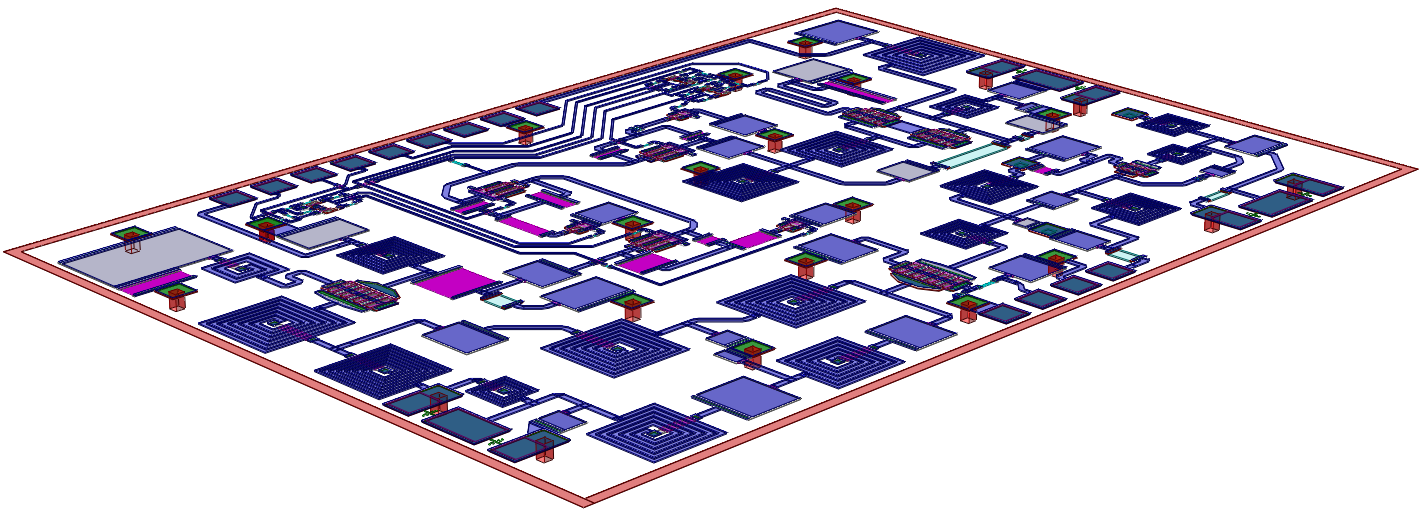
\includegraphics[width=1.0\textwidth]{fig/front_v3}

\vfill
\begin{tabular}{ll}
	Supervisors: & Niklas Billström \\
				 & Christian Fager \\
				 & \\
	Examiner:	 & Christian Fager \\
				 & Microwave Electronics Laboratory, MC2 \\
				 & Chalmers University of Technology \\
				 & Göteborg
\end{tabular}
\end{center}

\newpage	
%\clearpage
%\thispagestyle{empty}

\selectlanguage{english}
\begin{abstract}
	An S band, high-linearity down-converter is implemented using a \unit[0.25]{\mum} GaAs MMIC pHEMT-process. Using UMS' PPH25 process, an unbalanced FET resistive mixer with a lumped diplexer and an integrated square-wave LO-drive performs the down-converting. The produced narrowband IF-signal is then  amplified twice, first in an LNA and then in a highly linear amplifier. The chip has a dynamic attenuation range of \unit[10.5]{dB} and offers a maximum gain of \unit[15]{dB}. The input \unit[1]{dB}-compression point at nominal gain is \unit[10]{dBm} which estimates input $IP_3$ to \unit[20]{dBm}. The noise figure at nominal gain is \unit[11]{dB}.
	
	The chip offers down-converting of RF-frequencies between \unit[2.4 and 3.4]{GHz} for input LO-signals of \unit[-4--0]{dBm} and an image rejection of \unit[40]{dBc}. The chip size is \unit[2.9$\times$3.4]{mm}, and it is designed to fit in a \unit[4$\times$5]{mm} QFN-capsule and consumes \unit[1.0]{W} of DC power. Three control signals govern the dynamic attenuation with an LSB of \unit[1.6]{dB}.
	
	Comparative studies regarding mixer topologies and process technologies are performed. The choice of a single cold FET resistive mixer type is motivated by its linearity, small size and simplicity. A medium-power pHEMT process is chosen, as this provides improved linearity of the amplifiers as well as acceptable noise features given the requirements.

\end{abstract}

%\setcounter{page}{4}
%\newpage
\selectlanguage{swedish}
\begin{abstract}
	En linjär blandare för S-bandet har implementerats med en \unit[0.25]{\mum} GaAs MMIC pHEMT-process. För nedkonvertering används en obalanserad resistiv FET-mixer som bygger på en diplexer och en integrerad fyrkantsformad LO-signal. Den nedblandade IF-signalen förstärks två gånger, först i en lågbrusförstärkare och sedan i en effektförstärkare. Chippet har en dynamisk dämpning på \unit[10.5]{dB} och har \unit[15]{dB} maximal förstärkning. Ingångs-$P_{1dB}$ är \unit[10]{dBm}, vilket ger ett uppskattat ingångs-$IP_3$ på \unit[20]{dBm}. Vid nominell förstärkning är brusfaktorn \unit[11]{dB}.
	
Chippet klarar nedblandning av RF-frekvenser mellan \unit[2.9 och 3.4]{GHz} för LO-effekter \unit[-4--0]{dBm} och dämpning av spegelfrekvenserna med minst \unit[40]{dBc}. Chippet är designat för montering i en \unit[4$\times$5]{mm} QFN-kapsel och förbrukar \unit[1.0]{W}. Tre kontrollsignaler styr den dynamiska dämpningen med \unit[1.6]{dB} LSB.

Jämförelsestudier av blandartopologier och processval har genomförts. Blandaren är vald på grund av dess linjäritet, mindre storlek och enkelhet. UMS PPH25 process har valts då den klarar hög effekt och därmed mer linjära förstärkare såväl som acceptabla brusförhållanden givet design\-specifikationen.

	
	
\end{abstract}

\selectlanguage{english}
\newpage
\clearpage
%\thispagestyle{empty}
\section*{Preface}
	This report concludes our master's thesis work on monolithic microwave integrated circuit down-converter design. It is the degree project for our Master of Science in Engineering Physics at Chalmers University of Technology. The work has been carried out at Saab Electronic Defence Systems (former Saab Microwave) in Mölndal, Sweden, in the fall of 2010.
	
	First and foremost we would like to thank our supervisor at Saab, Niklas Billström, for his guidance during our project and for an unceasing patience. We thank our boss, Karin Adebahr, for her early faith in our abilities. We would also like to thank Simon Kristiansson, Joakim Nilsson, Peter Karlsson and the rest of the IC-design department at Saab for input during our work.
	
	Moreover, we would like to thank our supervisor and examiner at Chalmers Microwave Electronics Laboratory, Christian Fager, for his support during the project.\\[1cm]

\hfill
\begin{tabular}{ l }
Richard Abrahamsson \\
Anders Bennehag \\
Göteborg \today
\end{tabular}
